\textbf{Parámetros iniciales:}

\begin{itemize}
    \item Frecuencia de muestreo: $F_s = 8000$ Hz
    \item Periodo de muestreo: $T = \frac{1}{F_s} = \frac{1}{8000} = 125\;\mu$s
    \item Frecuencia de corte pasa bajas: $f_c = 85$ Hz
    \item Frecuencia de corte pasa altas: $f_c = 480$ Hz
    \item Frecuencia central (pasa banda): $f_o = 580$ Hz
    \item Ancho de banda (pasa banda): $BW = 45$ Hz
    \item Número de muestras por captura: 500
    \item Tipo de filtro: Butterworth IIR
\end{itemize}

% ==================================================================
\subsection{Diseño del Filtro Pasa Bajas de Primer Orden}
% ==================================================================


El prototipo analógico Butterworth de primer orden tiene la función de transferencia:

\begin{equation}
    H(s) = \frac{\omega_c}{s + \omega_c}
    \label{eq:lp_analog}
\end{equation}


Se calcula la frecuencia de corte pre-distorsionada para compensar el efecto de la transformación bilineal:

\begin{equation}
    \Omega_c = 2 F_s \tan\!\left(\frac{\pi f_c}{F_s}\right) = 2(8000)\tan\!\left(\frac{\pi \cdot 85}{8000}\right) = 16000\,\tan(0.03337)
\end{equation}

\begin{equation}
    \Omega_c = 16000 \times 0.033386 = 534.18 \;\text{rad/s}
\end{equation}

\textbf{Aplicación de la Transformación Bilineal}

Sustituyendo $s = 2F_s\cdot\frac{z-1}{z+1}$ en $H(s)$ con $\omega_c$ reemplazado por $\Omega_c$:

\begin{equation}
    H(z) = \frac{\Omega_c}{2F_s \cdot \frac{z-1}{z+1} + \Omega_c}
\end{equation}

Multiplicando numerador y denominador por $(z+1)$:

\begin{equation}
    H(z) = \frac{\Omega_c(z+1)}{2F_s(z-1) + \Omega_c(z+1)}
\end{equation}

Expandiendo el denominador:

\begin{equation}
    H(z) = \frac{\Omega_c(z+1)}{(2F_s + \Omega_c)\,z + (\Omega_c - 2F_s)}
\end{equation}

Dividiendo todo entre $(2F_s + \Omega_c)$:

\begin{equation}
    H(z) = \frac{\frac{\Omega_c}{2F_s + \Omega_c}(z + 1)}{z - \frac{2F_s - \Omega_c}{2F_s + \Omega_c}}
\end{equation}

\textbf{Cálculo de los Coeficientes}

\begin{align}
    A_0 = A_1 &= \frac{\Omega_c}{2F_s + \Omega_c} = \frac{534.18}{16000 + 534.18} = \frac{534.18}{16534.18} \approx 0.03230 \\[6pt]
    A_2 &= 0 \\[6pt]
    B_1 &= \frac{2F_s - \Omega_c}{2F_s + \Omega_c} = \frac{16000 - 534.18}{16534.18} = \frac{15465.82}{16534.18} \approx 0.93540 \\[6pt]
    B_2 &= 0
\end{align}

\textbf{Ganancia en DC}

En DC ($z = 1$):

\begin{equation}
    H(1) = \frac{A_0 + A_1}{1 - B_1} = \frac{0.03230 + 0.03230}{1 - 0.93540} = \frac{0.06460}{0.06460} = 1.0 \;\checkmark
\end{equation}

Esto confirma que el filtro tiene ganancia unitaria en DC, como se espera de un pasa bajas.

\subsubsection{Función de Transferencia:}

\begin{equation}
    \boxed{H(z) = \frac{0.03230\,z + 0.03230}{z - 0.93540} = \frac{0.03230(1 + z^{-1})}{1 - 0.93540\,z^{-1}}}
    \label{eq:lp_Hz}
\end{equation}

\textbf{Diagrama de Bloques}

\begin{figure}[H]
    \centering
    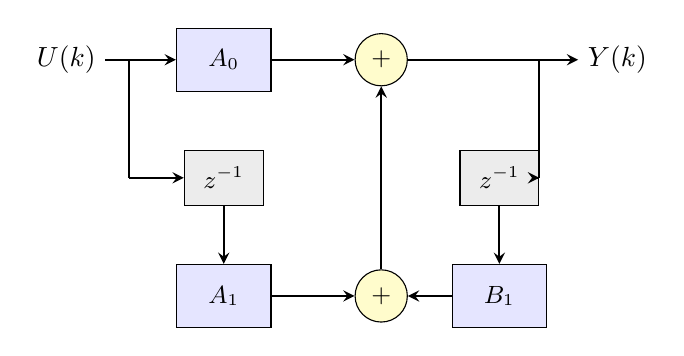
\begin{tikzpicture}[
        block/.style={rectangle, draw, fill=blue!10, minimum width=1.2cm, minimum height=0.8cm, font=\small},
        sum/.style={circle, draw, fill=yellow!20, minimum size=0.6cm, font=\small},
        delay/.style={rectangle, draw, fill=gray!15, minimum width=1cm, minimum height=0.7cm, font=\small},
        line/.style={draw, thick, ->, >=stealth}
    ]
        \node (input) at (0,0) {$U(k)$};
        \node[block] (a0) at (2, 0) {$A_0$};
        \node[sum] (s1) at (4, 0) {$+$};
        \node (output) at (7, 0) {$Y(k)$};

        \node[delay] (z1u) at (2, -1.5) {$z^{-1}$};
        \node[block] (a1) at (2, -3) {$A_1$};

        \node[delay] (z1y) at (5.5, -1.5) {$z^{-1}$};
        \node[block] (b1) at (5.5, -3) {$B_1$};
        \node[sum] (s2) at (4, -3) {$+$};

        \draw[line] (input) -- (a0);
        \draw[line] (a0) -- (s1);
        \draw[line] (s1) -- node[above] {} (output);

        \draw[thick] (0.8, 0) -- (0.8, -1.5);
        \draw[line] (0.8, -1.5) -- (z1u);
        \draw[line] (z1u) -- (a1);
        \draw[line] (a1) -- (s2);
        \draw[line] (s2) -- (s1);

        \draw[thick] (6, 0) -- (6, -1.5);
        \draw[line] (6, -1.5) -- (z1y);
        \draw[line] (z1y) -- (b1);
        \draw[line] (b1) -- (s2);
    \end{tikzpicture}
    \caption{Diagrama de bloques del filtro pasa bajas de primer orden (Forma Directa I).}
    \label{fig:bloques_lp}
\end{figure}

\subsubsection{Frecuencias de entradas en matlab:}

\begin{table}[H]
    \centering
    \caption{Frecuencias de prueba para el filtro pasa bajas ($f_c = 85$ Hz)}
    \begin{tabular}{|c|c|l|}
        \hline
        \rowcolor{subheadblue}\textbf{Frecuencia} & \textbf{Relación con $f_c$} & \textbf{Comportamiento esperado} \\
        \hline
        20 Hz & $f \ll f_c$ & Paso sin atenuación \\
        \hline
        50 Hz & $f < f_c$ & Paso con mínima atenuación, curva exponencial visible \\
        \hline
        85 Hz & $f = f_c$ & Atenuación de $-3$ dB (70.7\%) \\
        \hline
        200 Hz & $f > f_c$ & Atenuación significativa \\
        \hline
        500 Hz & $f \gg f_c$ & Atenuación fuerte \\
        \hline
    \end{tabular}
\end{table}

% ==================================================================
\subsection{Diseño del Filtro Pasa Altas de Primer Orden}
% ==================================================================


El prototipo analógico Butterworth pasa altas de primer orden:

\begin{equation}
    H(s) = \frac{s}{s + \omega_c}
    \label{eq:hp_analog}
\end{equation}

Para el filtro pasa altas se selecciona $f_c = 480$ Hz. La frecuencia pre-distorsionada es:

\begin{equation}
    \Omega_c = 2 F_s \tan\!\left(\frac{\pi \cdot 480}{8000}\right) = 16000\,\tan(0.18850) = 16000 \times 0.19089 = 3054.24 \;\text{rad/s}
\end{equation}

Sustituyendo en la transformación bilineal:

\begin{equation}
    H(z) = \frac{2F_s \cdot \frac{z-1}{z+1}}{2F_s \cdot \frac{z-1}{z+1} + \Omega_c}
\end{equation}

Multiplicando por $(z+1)$:

\begin{equation}
    H(z) = \frac{2F_s(z-1)}{2F_s(z-1) + \Omega_c(z+1)} = \frac{2F_s(z-1)}{(2F_s + \Omega_c)\,z + (\Omega_c - 2F_s)}
\end{equation}

Dividiendo entre $(2F_s + \Omega_c)$:

\begin{equation}
    H(z) = \frac{\frac{2F_s}{2F_s + \Omega_c}(z - 1)}{z - \frac{2F_s - \Omega_c}{2F_s + \Omega_c}}
\end{equation}

\textbf{Cálculo de los Coeficientes}

\begin{align}
    A_0 &= \frac{2F_s}{2F_s + \Omega_c} = \frac{16000}{19054.24} \approx 0.83970 \\[6pt]
    A_1 &= -A_0 = -0.83970 \\[6pt]
    A_2 &= 0 \\[6pt]
    B_1 &= \frac{2F_s - \Omega_c}{2F_s + \Omega_c} = 0.67940 \\[6pt]
    B_2 &= 0
\end{align}

\textbf{Ganancia en DC y Nyquist}

En DC ($z = 1$):
\begin{equation}
    H(1) = \frac{A_0 + A_1}{1 - B_1} = \frac{0.83970 - 0.83970}{1 - 0.67940} = \frac{0}{0.32060} = 0 \;\checkmark
\end{equation}

En Nyquist ($z = -1$):
\begin{equation}
    H(-1) = \frac{A_0(-1) + A_1}{-1 - (-B_1)} = \frac{-0.83970 - 0.83970}{-1 - 0.67940} = \frac{-1.67940}{-1.67940} = 1.0 \;\checkmark
\end{equation}

\textbf{Función de Transferencia Final}

\begin{equation}
    \boxed{H(z) = \frac{0.83970\,z - 0.83970}{z - 0.67940} = \frac{0.83970(1 - z^{-1})}{1 - 0.67940\,z^{-1}}}
    \label{eq:hp_Hz}
\end{equation}

\textbf{Diagrama de Bloques}

\begin{figure}[H]
    \centering
    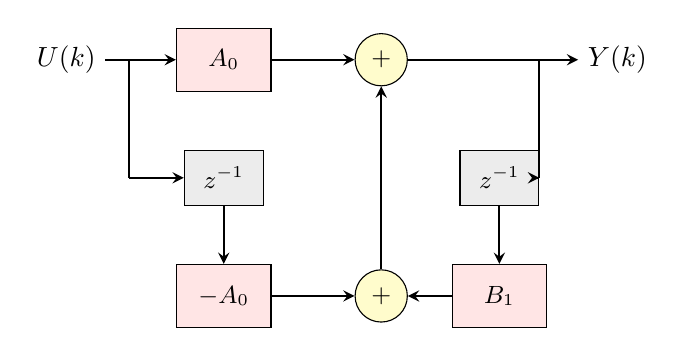
\begin{tikzpicture}[
        block/.style={rectangle, draw, fill=red!10, minimum width=1.2cm, minimum height=0.8cm, font=\small},
        sum/.style={circle, draw, fill=yellow!20, minimum size=0.6cm, font=\small},
        delay/.style={rectangle, draw, fill=gray!15, minimum width=1cm, minimum height=0.7cm, font=\small},
        line/.style={draw, thick, ->, >=stealth}
    ]
        \node (input) at (0,0) {$U(k)$};
        \node[block] (a0) at (2, 0) {$A_0$};
        \node[sum] (s1) at (4, 0) {$+$};
        \node (output) at (7, 0) {$Y(k)$};

        \node[delay] (z1u) at (2, -1.5) {$z^{-1}$};
        \node[block] (a1) at (2, -3) {$-A_0$};

        \node[delay] (z1y) at (5.5, -1.5) {$z^{-1}$};
        \node[block] (b1) at (5.5, -3) {$B_1$};
        \node[sum] (s2) at (4, -3) {$+$};

        \draw[line] (input) -- (a0);
        \draw[line] (a0) -- (s1);
        \draw[line] (s1) -- node[above] {} (output);

        \draw[thick] (0.8, 0) -- (0.8, -1.5);
        \draw[line] (0.8, -1.5) -- (z1u);
        \draw[line] (z1u) -- (a1);
        \draw[line] (a1) -- (s2);
        \draw[line] (s2) -- (s1);

        \draw[thick] (6, 0) -- (6, -1.5);
        \draw[line] (6, -1.5) -- (z1y);
        \draw[line] (z1y) -- (b1);
        \draw[line] (b1) -- (s2);
    \end{tikzpicture}
    \caption{Diagrama de bloques del filtro pasa altas de primer orden (Forma Directa I).}
    \label{fig:bloques_hp}
\end{figure}

\textbf{Frecuencias de entradas en matlab:}

\begin{table}[H]
    \centering
    \caption{Frecuencias de prueba para el filtro pasa altas ($f_c = 480$ Hz)}
    \begin{tabular}{|c|c|l|}
        \hline
        \rowcolor{subheadblue}\textbf{Frecuencia} & \textbf{Relación con $f_c$} & \textbf{Comportamiento esperado} \\
        \hline
        50 Hz & $f \ll f_c$ & Atenuación fuerte \\
        \hline
        200 Hz & $f < f_c$ & Atenuación significativa \\
        \hline
        480 Hz & $f = f_c$ & Atenuación de $-3$ dB (70.7\%) \\
        \hline
        1000 Hz & $f > f_c$ & Paso con mínima atenuación \\
        \hline
        2000 Hz & $f \gg f_c$ & Paso sin atenuación \\
        \hline
    \end{tabular}
\end{table}

% ==================================================================
\subsection{Filtro Pasa Banda de Segundo Orden}
% ==================================================================

\textbf{Parámetros}

\begin{itemize}
    \item Frecuencia central: $f_o = 580$ Hz
    \item Ancho de banda: $BW = 45$ Hz
    \item Frecuencias de corte: $f_{c1} = f_o - BW/2 = 557.5$ Hz, \quad $f_{c2} = f_o + BW/2 = 602.5$ Hz
\end{itemize}

Se aplica pre-warping a ambas frecuencias de corte:

\begin{align}
    \Omega_1 &= 2F_s\,\tan\!\left(\frac{\pi f_{c1}}{F_s}\right) = 16000\,\tan\!\left(\frac{\pi \cdot 557.5}{8000}\right) = 16000\,\tan(0.21893) \\[4pt]
    &= 16000 \times 0.22237 = 3557.9 \;\text{rad/s} \\[8pt]
    \Omega_2 &= 2F_s\,\tan\!\left(\frac{\pi f_{c2}}{F_s}\right) = 16000\,\tan\!\left(\frac{\pi \cdot 602.5}{8000}\right) = 16000\,\tan(0.23658) \\[4pt]
    &= 16000 \times 0.24203 = 3872.5 \;\text{rad/s}
\end{align}

\begin{align}
    \Omega_0 &= \sqrt{\Omega_1 \cdot \Omega_2} = \sqrt{3557.9 \times 3872.5} = \sqrt{13\,779\,000} \approx 3712.0 \;\text{rad/s} \\[6pt]
    \Omega_0^2 &\approx 13\,778\,944 \\[6pt]
    BW_w &= \Omega_2 - \Omega_1 = 3872.5 - 3557.9 = 314.6 \;\text{rad/s}
\end{align}

\textbf{Función de Transferencia del Pasa Banda}

El prototipo analógico Butterworth pasa banda de segundo orden:

\begin{equation}
    H(s) = \frac{BW_w \cdot s}{s^2 + BW_w \cdot s + \Omega_0^2}
\end{equation}

Aplicando la transformación bilineal $s = K\,\frac{z-1}{z+1}$ con $K = 2F_s = 16000$:

\begin{equation}
    H(z) = \frac{BW_w \cdot K \cdot \frac{z-1}{z+1}}{\left(K\,\frac{z-1}{z+1}\right)^{\!2} + BW_w \cdot K \cdot \frac{z-1}{z+1} + \Omega_0^2}
\end{equation}

Multiplicando numerador y denominador por $(z+1)^2$:

\begin{equation}
    H(z) = \frac{BW_w \cdot K\,(z^2 - 1)}{K^2(z-1)^2 + BW_w \cdot K\,(z^2-1) + \Omega_0^2(z+1)^2}
\end{equation}

\subsubsection{Expansión del Denominador}

\begin{align}
    K^2(z-1)^2 &= K^2\,z^2 - 2K^2\,z + K^2 \\
    BW_w \cdot K\,(z^2-1) &= BW_w \cdot K\,z^2 - BW_w \cdot K \\
    \Omega_0^2(z+1)^2 &= \Omega_0^2\,z^2 + 2\Omega_0^2\,z + \Omega_0^2
\end{align}

Sumando término a término:

\begin{equation}
    D(z) = \underbrace{(K^2 + BW_w K + \Omega_0^2)}_{\alpha}\,z^2 + \underbrace{(-2K^2 + 2\Omega_0^2)}_{\beta}\,z + \underbrace{(K^2 - BW_w K + \Omega_0^2)}_{\gamma}
\end{equation}

Sustituyendo valores numéricos ($K = 16000$, $K^2 = 256\,000\,000$):

\begin{align}
    \alpha &= 256\,000\,000 + 5\,033\,600 + 13\,778\,944 = 274\,812\,544 \\
    \beta  &= -512\,000\,000 + 27\,557\,888 = -484\,442\,112 \\
    \gamma &= 256\,000\,000 - 5\,033\,600 + 13\,778\,944 = 264\,745\,344
\end{align}

\textbf{Coeficientes del Filtro Discreto}

Dividiendo numerador y denominador entre $\alpha$:

\begin{align}
    A_0 &= \frac{BW_w \cdot K}{\alpha} = \frac{314.6 \times 16000}{274\,812\,544} = \frac{5\,033\,600}{274\,812\,544} \approx 0.01832 \\[6pt]
    A_1 &= 0 \\[6pt]
    A_2 &= -A_0 = -0.01832 \\[6pt]
    B_1 &= -\frac{\beta}{\alpha} = -\frac{-484\,442\,112}{274\,812\,544} = \frac{484\,442\,112}{274\,812\,544} \approx 1.76283 \\[6pt]
    B_2 &= -\frac{\gamma}{\alpha} = -\frac{264\,745\,344}{274\,812\,544} \approx -0.96337
\end{align}

\textbf{Verificación}

En DC ($z = 1$):
\begin{equation}
    H(1) = \frac{A_0(1) + 0 + A_2(1)}{1 - B_1 - B_2} = \frac{0.01832 - 0.01832}{1 - 1.76283 + 0.96337} = \frac{0}{0.20054} = 0 \;\checkmark
\end{equation}

En Nyquist ($z = -1$):
\begin{equation}
    H(-1) = \frac{A_0 + A_2}{1 + B_1 - B_2} = \frac{0}{1 + 1.76283 + 0.96337} = 0 \;\checkmark
\end{equation}

El filtro pasa banda rechaza correctamente tanto las señales DC como las de frecuencia Nyquist.

\subsubsection{Función de Transferencia Final}

\begin{equation}
    \boxed{H(z) = \frac{0.01832\,z^2 - 0.01832}{z^2 - 1.76283\,z + 0.96337} = \frac{0.01832(1 - z^{-2})}{1 - 1.76283\,z^{-1} + 0.96337\,z^{-2}}}
    \label{eq:bp_Hz}
\end{equation}

\textbf{Diagrama de Bloques}

\begin{figure}[H]
    \centering
    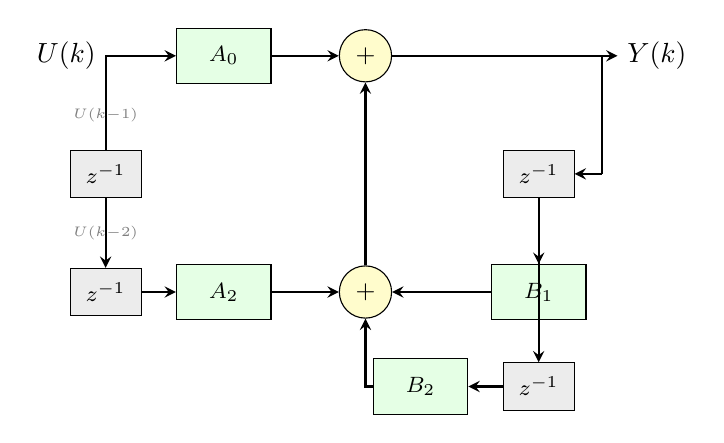
\begin{tikzpicture}[
        block/.style={rectangle, draw, fill=green!10, minimum width=1.2cm, minimum height=0.7cm, font=\footnotesize},
        sum/.style={circle, draw, fill=yellow!20, minimum size=0.55cm, font=\small},
        delay/.style={rectangle, draw, fill=gray!15, minimum width=0.9cm, minimum height=0.6cm, font=\footnotesize},
        line/.style={draw, thick, ->, >=stealth}
    ]
        \node (input) at (0,0) {$U(k)$};
        \node[block] (a0) at (2, 0) {$A_0$};
        \node[sum] (s1) at (3.8, 0) {$+$};
        \node (output) at (7.5, 0) {$Y(k)$};

        % Rama U(k-2)
        \node[delay] (z1u) at (0.5, -1.5) {$z^{-1}$};
        \node[delay] (z2u) at (0.5, -3) {$z^{-1}$};
        \node[block] (a2) at (2, -3) {$A_2$};

        % Ramas Y(k-1), Y(k-2)
        \node[delay] (z1y) at (6, -1.5) {$z^{-1}$};
        \node[block] (b1) at (6, -3) {$B_1$};
        \node[delay] (z2y) at (6, -4.2) {$z^{-1}$};
        \node[block] (b2) at (4.5, -4.2) {$B_2$};

        \node[sum] (s2) at (3.8, -3) {$+$};

        \draw[line] (input) -- (a0);
        \draw[line] (a0) -- (s1);
        \draw[line] (s1) -- (output);

        \draw[thick] (0.5, 0) -- (z1u);
        \draw[line] (z1u) -- (z2u);
        \draw[line] (z2u) -- (a2);
        \draw[line] (a2) -- (s2);
        \draw[line] (s2) -- (s1);

        \draw[thick] (6.8, 0) -- (6.8, -1.5);
        \draw[line] (6.8, -1.5) -- (z1y);
        \draw[line] (z1y) -- (b1);
        \draw[line] (b1) -- (s2);
        \draw[line] (z1y.south) -- (z2y);
        \draw[line] (z2y) -- (b2);
        \draw[line] (b2.west) -| (s2.south);

        \node[font=\tiny, gray] at (0.5, -0.75) {$U(k{-}1)$};
        \node[font=\tiny, gray] at (0.5, -2.25) {$U(k{-}2)$};
    \end{tikzpicture}
    \caption{Diagrama de bloques del filtro pasa banda de segundo orden (Forma Directa I). Nota: $A_1 = 0$, por lo que no hay rama para $U(k{-}1)$.}
    \label{fig:bloques_bp}
\end{figure}

% ==================================================================
\subsection{Coeficientes de todos los filtros;}
% ==================================================================

\begin{table}[H]
    \centering
    \caption{Coeficientes de los filtros IIR diseñados ($F_s = 8000$ Hz)}
    \label{tab:coeficientes}
    \begin{tabular}{|l|c|c|c|}
        \hline
        \rowcolor{headblue}\textcolor{white}{\textbf{Coeficiente}} & \textcolor{white}{\textbf{Pasa Bajas}} & \textcolor{white}{\textbf{Pasa Altas}} & \textcolor{white}{\textbf{Pasa Banda}} \\
        \hline
        $f_c$ o $f_o$ & 85 Hz & 480 Hz & 580 Hz \\
        \hline
        $BW$ & --- & --- & 45 Hz \\
        \hline
        $A_0$ & $0.03230$ & $0.83970$ & $0.01832$ \\
        \hline
        $A_1$ & $0.03230$ & $-0.83970$ & $0.0$ \\
        \hline
        $A_2$ & $0.0$ & $0.0$ & $-0.01832$ \\
        \hline
        $B_1$ & $0.93540$ & $0.67940$ & $1.76283$ \\
        \hline
        $B_2$ & $0.0$ & $0.0$ & $-0.96337$ \\
        \hline
    \end{tabular}
\end{table}

\begin{itemize}
    \item \textbf{Pasa Bajas} ($f_c = 85$ Hz): Primer orden, ganancia unitaria en DC, atenuación de $-3$~dB en $f_c$. Con $f_c$ baja, la señal de salida presenta una curva exponencial visible al filtrar ondas cuadradas. Probarlo con 50~Hz (paso con forma exponencial), 85~Hz ($-3$~dB) y 500~Hz (atenuación fuerte).
    \item \textbf{Pasa Altas} ($f_c = 480$ Hz): Primer orden, rechazo total en DC, ganancia unitaria en Nyquist. Elimina componentes de baja frecuencia, dejando solo transitorios (flancos) de la onda cuadrada. Probarlo con 50~Hz (atenuación), 480~Hz ($-3$~dB) y 2000~Hz (paso).
    \item \textbf{Pasa Banda} ($f_o = 580$ Hz, $BW = 45$ Hz): Segundo orden, selectivo en frecuencia. Extrae la componente a 580~Hz de la señal, produciendo una salida sinusoidal. Probarlo con 580~Hz (paso), 50~Hz (atenuación) y 2000~Hz (atenuación).
\end{itemize}

% ==================================================================
\subsection{Diagrama de Conexión del Circuito}
% ==================================================================

\begin{figure}[H]
    \centering
    \begin{tikzpicture}[scale=0.85, transform shape]
        \picoboard

        % HC-05 Bluetooth Module
        \node[draw, thick, fill=blue!10, minimum width=2.5cm, minimum height=2cm, align=center, font=\small\sffamily] (bt) at (-4, -1.35) {HC-05\\Bluetooth\\460800 baud};

        % Conexiones HC-05 a Pico
        \draw[blue, thick, ->] (bt.east) ++(0, 0.4) -- (P1) node[midway, above, font=\tiny\sffamily] {TX $\to$ GP0 (RX)};
        \draw[red!70!black, thick, <-] (bt.east) ++(0, -0.4) -- (P2) node[midway, below, font=\tiny\sffamily] {RX $\leftarrow$ GP1 (TX)};

        % Cable Pin3 -> Pin26 (ADC) - Ruta limpia por abajo
        \draw[green!60!black, ultra thick, dashed]
            (P5) -- ++(-0.6, 0) -- ++(0, -8.5) -- ++(6.2, 0) -- ++(0, 6.25) -- (P31);

        % Etiqueta del cable
        \node[draw, fill=green!10, font=\tiny\sffamily, align=center, rounded corners] at (2, -11.2) {Cable: GP3 $\to$ GP26};

        % GND connections
        \draw[black, thick] (bt.south) |- ([yshift=-0.8cm]PGND) node[pos=0.75, above, font=\tiny\sffamily] {GND} -- (PGND);

        % Etiquetas
        \node[font=\scriptsize\sffamily, blue, align=center] at (-4, -3.5) {Hacia PC\\via Bluetooth};

        % Onda cuadrada label
        \node[font=\tiny\sffamily, orange, align=center] at (-2, -2.7) {Onda cuadrada\\(toggle manual)};

        % ADC label
        \node[draw, fill=purple!10, font=\tiny\sffamily, align=center, rounded corners] at (6.5, -3.8) {ADC\\Entrada\\analógica};
        \draw[purple, thick, ->] (5.8, -4.0) -- (P31);

    \end{tikzpicture}
    \caption{Diagrama de conexión del circuito: Raspberry Pi Pico 2W con módulo HC-05 y lazo de retroalimentación.}
    \label{fig:circuito}
\end{figure}

\textbf{Funcionamiento del circuito:}
\begin{enumerate}
    \item MATLAB envía los coeficientes del filtro $(A_0, A_1, A_2, B_1, B_2)$ y la frecuencia de la señal de prueba a través de Bluetooth.
    \item La Pico configura la frecuencia de la onda cuadrada generada por toggle manual en el hilo del Core~2.
    \item Al recibir el comando de captura (\texttt{0x52}), el Core~1 ejecuta la ecuación en diferencias a 8~kHz durante 500 muestras.
    \item La onda cuadrada generada en el Pin~3 se conecta externamente al Pin~26 (ADC), sirviendo como señal de entrada.
    \item Los vectores de entrada $U(k)$ y salida $Y(k)$ se envían de vuelta a MATLAB para su visualización.
\end{enumerate}

% ==================================================================
\subsection{Protocolo de Comunicación UART}
% ==================================================================

La comunicación entre MATLAB y la Raspberry Pi Pico se realiza mediante UART a 460800 baudios a través del módulo HC-05. Se definen dos tipos de tramas:

MATLAB envía una trama de 25 bytes con la siguiente estructura:

\begin{table}[H]
    \centering
    \caption{Estructura de la trama de coeficientes}
    \begin{tabular}{|c|c|c|l|}
        \hline
        \rowcolor{subheadblue}\textbf{Byte(s)} & \textbf{Campo} & \textbf{Formato} & \textbf{Descripción} \\
        \hline
        0 & Encabezado & \texttt{0x55} (``U'') & Identificador de trama \\
        \hline
        1--4 & $A_0$ & float32 LE & Coeficiente de $U(k)$ \\
        \hline
        5--8 & $A_1$ & float32 LE & Coeficiente de $U(k{-}1)$ \\
        \hline
        9--12 & $A_2$ & float32 LE & Coeficiente de $U(k{-}2)$ \\
        \hline
        13--16 & $B_1$ & float32 LE & Coeficiente de $Y(k{-}1)$ \\
        \hline
        17--20 & $B_2$ & float32 LE & Coeficiente de $Y(k{-}2)$ \\
        \hline
        21--24 & FREQ & float32 LE & Frecuencia de prueba (Hz) \\
        \hline
    \end{tabular}
\end{table}


MATLAB envía el byte \texttt{0x52} para iniciar la captura de datos.

% ==================================================================
\subsection{Explicación del Código:}
% ==================================================================


\begin{lstlisting}[language={[LAB]Python}, caption={Código MicroPython del simulador de filtros IIR}, label={lst:main_code}]
import machine
machine.freq(300_000_000)  # Overclock a 300 MHz

from machine import Pin, ADC, UART
from time import sleep_ms, sleep_us, ticks_us, ticks_diff, ticks_add
import _thread
import struct

ADC0 = ADC(Pin(26))
Pin3 = Pin(3, Pin.OUT)
UART0 = UART(0, baudrate=460800, tx=Pin(0), rx=Pin(1))

conversion_factor = 3.3 / 65535
MUESTRAS = 1000
ENTRADAS = [0]*MUESTRAS
SALIDAS  = [0]*MUESTRAS
En_Bytes = bytearray(4000)

CTE_A0, CTE_A1, CTE_A2 = 0.0303, 0.0303, 0.0
CTE_B1, CTE_B2 = 0.9394, 0.0
FREQ = 50
PERIODO = 1/FREQ
HALF = int((PERIODO*1000000)/2)

def Onda_Cuadrada():
    while True:
        Pin3.on()
        sleep_us(HALF)
        Pin3.off()
        sleep_us(HALF)

@micropython.native
def capturar(a0, a1, a2, b1, b2):
    uk = uk1 = uk2 = 0.0
    yk = yk1 = yk2 = 0.0
    adc = ADC0.read_u16
    cf  = conversion_factor
    ent = ENTRADAS
    sal = SALIDAS
    _tu = ticks_us
    _td = ticks_diff
    _ta = ticks_add
    _su = sleep_us

    t_next = _tu()
    for i in range(500):
        yk = a0*uk + a1*uk1 + a2*uk2 + b1*yk1 + b2*yk2
        uk2 = uk1
        uk1 = uk
        yk2 = yk1
        yk1 = yk
        uk = adc() * cf
        ent[i] = uk
        sal[i] = yk
        t_next = _ta(t_next, 125)
        dt = _td(t_next, _tu())
        if dt > 0:
            _su(dt)

_thread.start_new_thread(Onda_Cuadrada, ())

while True:
    if UART0.any() > 0:
        sleep_ms(100)
        LLAVE = UART0.read()
        if LLAVE and LLAVE[0] == 0x55:
            # Decodificar 6 flotantes IEEE 754 LE
            CTE_A0 = struct.unpack('<f', LLAVE[1:5])[0]
            CTE_A1 = struct.unpack('<f', LLAVE[5:9])[0]
            CTE_A2 = struct.unpack('<f', LLAVE[9:13])[0]
            CTE_B1 = struct.unpack('<f', LLAVE[13:17])[0]
            CTE_B2 = struct.unpack('<f', LLAVE[17:21])[0]
            FREQ   = struct.unpack('<f', LLAVE[21:25])[0]
            HALF   = int((1/FREQ * 1000000) / 2)
        if LLAVE and 0x52 in LLAVE:
            capturar(CTE_A0, CTE_A1, CTE_A2, CTE_B1, CTE_B2)
            for i in range(500):
                struct.pack_into('f', En_Bytes, i*8, ENTRADAS[i])
                struct.pack_into('f', En_Bytes, i*8+4, SALIDAS[i])
            for j in range(0, 4000, 50):
                UART0.write(En_Bytes[j:j+50])
                sleep_ms(60)
\end{lstlisting}

\subsubsection{Configuración del Hardware}

\begin{lstlisting}[language=Python, caption={Configuración de la frecuencia del reloj}]
import machine
machine.freq(300_000_000)  # Overclock a 300 MHz
\end{lstlisting}

Se incrementa la frecuencia del procesador de 125 MHz (valor por defecto) a 300 MHz para mejorar la velocidad y precisión de los cálculos y del control de tiempo en la función \texttt{capturar()} a 8 kHz.

\begin{lstlisting}[language=Python, caption={Limpieza de PWM residual}]
# Limpiar cualquier PWM residual en Pin 3
try:
    from machine import PWM
    _p = PWM(Pin(3))
    _p.deinit()
except:
    pass
\end{lstlisting}

Limpia cualquier señal PWM que pudiera haber quedado configurada en el Pin 3 de ejecuciones anteriores. Esto evita conflictos porque el mismo pin se usará como salida digital GPIO.

\begin{lstlisting}[language=Python, caption={Inicialización de periféricos y comunicación}]
ADC0 = ADC(Pin(26))       # Entrada analógica en GP26
Pin3 = Pin(3, Pin.OUT)     # Salida digital para la onda cuadrada
UART0 = UART(0, baudrate=460800, tx=Pin(0), rx=Pin(1))  # Comunicación Bluetooth
\end{lstlisting}

\begin{itemize}
    \item \textbf{\texttt{ADC0}:} Convierte la señal analógica de entrada (proveniente del Pin 3 conectado externamente al Pin 26).
    \item \textbf{\texttt{Pin3}:} Genera la onda cuadrada que sirve como señal de prueba.
    \item \textbf{\texttt{UART0}:} Canal de comunicación serie con el módulo HC-05 a 460,800 baudios.
\end{itemize}


\subsubsection{Variables Globales}

\begin{lstlisting}[language=Python, caption={Definición de factores de conversión y buffers}]
conversion_factor = 3.3 / 65535   # Convierte lecturas ADC (0-65535) a voltios (0-3.3 V)
MUESTRAS = 1000
ENTRADAS = [0] * MUESTRAS         # Buffer para almacenar U(k)
SALIDAS  = [0] * MUESTRAS         # Buffer para almacenar Y(k)
En_Bytes = bytearray(4000)        # Espacio en memoria para enviar los datos por USB
\end{lstlisting}

Los buffers \texttt{ENTRADAS} y \texttt{SALIDAS} guardan temporalmente los datos obtenidos durante la captura antes de enviarlos. Por otro lado, \texttt{En\_Bytes} reserva un espacio fijo en memoria para transmitir los datos por USB, evitando retrasos o interrupciones durante la ejecución del sistema en tiempo real.


\begin{lstlisting}[language=Python, caption={Coeficientes del filtro y temporización de la onda cuadrada}]
# Coeficientes iniciales (pasa bajas, fc \approx 85 Hz)
CTE_A0, CTE_A1, CTE_A2 = 0.0303, 0.0303, 0.0
CTE_B1, CTE_B2 = 0.9394, 0.0
FREQ = 50           # Frecuencia inicial de la onda cuadrada (Hz)
PERIODO = 1/FREQ
HALF = int((PERIODO * 1_000_000) / 2)  # Semiperíodo en microsegundos
\end{lstlisting}


\begin{itemize}
    \item \textbf{\texttt{CTE\_A0}, \texttt{CTE\_A1}, \texttt{CTE\_A2}, \texttt{CTE\_B1}, \texttt{CTE\_B2}:} Coeficientes iniciales para la implementación de un filtro digital paso bajo con una frecuencia de corte ($f_c$) de aproximadamente 85 Hz.
    \item \textbf{\texttt{FREQ}:} Define la frecuencia inicial de la onda cuadrada, establecida por defecto en 50 Hz.
    \item \textbf{\texttt{PERIODO} y \texttt{HALF}:} Determinan matemáticamente el período de la señal y el semiperíodo (\texttt{HALF}) convertido a microsegundos, necesario para controlar con precisión los tiempos de conmutación del pin digital.
\end{itemize}

\subsubsection{Función Onda\_Cuadrada() - Núcleo 2 (hilo secundario)}

\begin{lstlisting}[language=Python, caption={Generación de señal en el hilo secundario}]
def Onda_Cuadrada():
    while True:
        Pin3.on()
        sleep_us(HALF)
        Pin3.off()
        sleep_us(HALF)
\end{lstlisting}

Genera una onda cuadrada con un ciclo de trabajo del 50\,\% en el \texttt{Pin3}. Esta función se ejecuta en el Núcleo 2 (\textit{Core 2}) de la Raspberry Pi Pico 2W usando la biblioteca \texttt{\_thread}, por lo que trabaja de manera independiente al programa principal.

El valor de \texttt{HALF}, que define el semiperíodo de la señal, se actualiza automáticamente cuando MATLAB envía una nueva frecuencia. Como \texttt{HALF} es una variable global que se revisa continuamente, la frecuencia de la onda puede cambiarse en tiempo real sin detener la ejecución del hilo secundario.

\subsubsection{Función \texttt{capturar()} - Motor del Filtro Digital}

\begin{lstlisting}[language=Python, caption={Declaración y decorador de la función principal}]
@micropython.native
def capturar(a0, a1, a2, b1, b2):
\end{lstlisting}

La instrucción \texttt{@micropython.native} hace que la función se ejecute como código máquina nativo en lugar de código interpretado, aumentando considerablemente su velocidad de ejecución.

\begin{lstlisting}[language=Python, caption={Inicialización de variables de estado}]
    # Inicialización de estados del filtro (condiciones iniciales = 0)
    uk = uk1 = uk2 = 0.0    # Muestras de entrada actuales y anteriores
    yk = yk1 = yk2 = 0.0    # Muestras de salida actuales y anteriores
\end{lstlisting}

\begin{lstlisting}[language=Python, caption={Optimización mediante referencias locales}]
    # Referencias locales para máximo rendimiento (evitar búsqueda de atributos globales)
    adc = ADC0.read_u16
    cf  = conversion_factor
    ent = ENTRADAS
    sal = SALIDAS
    _tu = ticks_us
    _td = ticks_diff
    _ta = ticks_add
    _su = sleep_us
\end{lstlisting}

Este método de guardar referencias en variables locales es una optimización importante en MicroPython, ya que acceder a variables locales es aproximadamente $4\times$ más rápido que acceder a variables globales o atributos de objetos.


\begin{lstlisting}[language=Python, caption={Bucle principal de procesamiento del filtro}]
    t_next = _tu()           # Marca de tiempo del inicio
    for i in range(500):
        # 1. APLICAR LA ECUACIÓN EN DIFERENCIAS 
        yk = a0*uk + a1*uk1 + a2*uk2 + b1*yk1 + b2*yk2
        
        # 2. ACTUALIZAR ESTADOS (desplazamiento de registros de retardo)
        uk2 = uk1
        uk1 = uk
        yk2 = yk1
        yk1 = yk
        
        # 3. LEER NUEVA MUESTRA DEL ADC
        uk = adc() * cf        # Convierte a voltios
        
        # 4. GUARDAR EN BUFFERS
        ent[i] = uk
        sal[i] = yk
        
        # 5. CONTROL DE TEMPORIZACIÓN (periodo exacto de 125 microsegundos = 8 kHz)
        t_next = _ta(t_next, 125)
        dt = _td(t_next, _tu())
        if dt > 0:
            _su(dt)            # Esperar el tiempo restante del periodo
\end{lstlisting}

La ecuación en diferencias implementada es la forma general:

$$Y(k) = A_0 \cdot U(k) + A_1 \cdot U(k-1) + A_2 \cdot U(k-2) + B_1 \cdot Y(k-1) + B_2 \cdot Y(k-2)$$

El control del tiempo es muy importante: en lugar de usar un \texttt{sleep\_us(125)} fijo (lo que podría generar errores por el tiempo que tarda el programa en ejecutarse), el sistema calcula cuánto tiempo falta para la siguiente muestra y solo espera ese intervalo restante. De esta manera, se mantiene un periodo de muestreo estable de 125 $\mu$s.

\subsubsection{Bucle Principal - Protocolo de Comunicación}

\begin{lstlisting}[language=Python, caption={Inicialización del hilo secundario y bucle principal}]
_thread.start_new_thread(Onda_Cuadrada, ())   # Lanzar generador de onda en Core 2

while True:
    if UART0.any() > 0:
        sleep_ms(100)          #  Espera a que se reciban todos los datos
        LLAVE = UART0.read()
\end{lstlisting}

\newpage
\textbf{Recepción de Coeficientes (datos \texttt{0x55})}

\begin{lstlisting}[language=Python, caption={Decodificación de los datos de coeficientes}]
        if LLAVE and LLAVE[0] == 0x55:
            # Decodificar 6 floats IEEE 754 little-endian (4 bytes cada uno)
            CTE_A0 = struct.unpack('<f', LLAVE[1:5])[0]
            CTE_A1 = struct.unpack('<f', LLAVE[5:9])[0]
            CTE_A2 = struct.unpack('<f', LLAVE[9:13])[0]
            CTE_B1 = struct.unpack('<f', LLAVE[13:17])[0]
            CTE_B2 = struct.unpack('<f', LLAVE[17:21])[0]
            FREQ   = struct.unpack('<f', LLAVE[21:25])[0]
            HALF   = int((1/FREQ * 1_000_000) / 2)    # Actualizar semiperiodo
\end{lstlisting}

Los 25 bytes recibidos tienen la siguiente estructura:

\begin{table}[hbt!]
\centering
\begin{tabular}{|c|c|l|}
\hline
\textbf{Byte(s)} & \textbf{Dato} & \textbf{Descripción} \\ \hline
0 & \texttt{0x55} & Código de inicio del mensaje \\ \hline
1--4 & \texttt{A0} & Valor decimal de tipo \texttt{float32} \\ \hline
5--8 & \texttt{A1} & Valor decimal de tipo \texttt{float32} \\ \hline
9--12 & \texttt{A2} & Valor decimal de tipo \texttt{float32} \\ \hline
13--16 & \texttt{B1} & Valor decimal de tipo \texttt{float32} \\ \hline
17--20 & \texttt{B2} & Valor decimal de tipo \texttt{float32} \\ \hline
21--24 & \texttt{FREQ} & Frecuencia en formato \texttt{float32} \\ \hline
\end{tabular}
\caption{Distribución de los datos recibidos y su significado.}
\label{tab:trama_0x55}
\end{table}


\textbf{Inicio de la Captura de Datos (\texttt{0x52})}

\begin{lstlisting}[language=Python, caption={Ejecución de captura y envío de datos}]
        if LLAVE and 0x52 in LLAVE:
            # Realizar la captura usando los coeficientes actuales
            capturar(CTE_A0, CTE_A1, CTE_A2, CTE_B1, CTE_B2)
            
            # Guardar U(k) y Y(k) en formato float32
            for i in range(500):
                struct.pack_into('f', En_Bytes, i*8,   ENTRADAS[i])
                struct.pack_into('f', En_Bytes, i*8+4, SALIDAS[i])
                
            # Enviar los datos en bloques de 50 bytes
            for j in range(0, 4000, 50):
                UART0.write(En_Bytes[j:j+50])
                sleep_ms(60)    # Espera para evitar sobrecargar el HC-05
\end{lstlisting}

La transmisión se realiza en bloques de 50 bytes con una pausa de 60 ms entre cada uno. Esto se hace para evitar que el módulo Bluetooth HC-05 se sature y pierda datos al recibir toda la información demasiado rápido.